

% #######################################

\documentclass[12pt, a4paper]{report}

% all the other includes etc. are done in the thesis.sty file.
\usepackage{style}
\usepackage{ifthen}
\usepackage{datetime}


\renewcommand{\dateseparator}{-} % The ISO standard uses hyphens

% Document title and type
\newcommand{\doctitle}{Thesis Title} % The title of the thesis
\newcommand{\doctype}{Master's Thesis} 
% PhD Thesis
% Master's Thesis
% Bachelor's Thesis
% Thesis
% Dissertation
% End of Studies Project Report
% Graduation Project Report
% ...

% Info about university
\newcommand{\department}{Computer Science and Communication Department} % department
\newcommand{\degree}{Research Master} % your degree (Licence, Bachelor, Applied Master, PhD, etc)
\newcommand{\major}{Computer Science} % your major (Mathematics, Chemistry, Biology, etc)
\newcommand{\defenseDate}{July 2020} % defence date

% Thesis author
\newcommand{\authorName}{Hugo Simon}

% Main supervisor
\newcommand{\supervisor}{R\'emi Bardenet}

% Co-supervisor. If you have only one supervisor, leave it as it is
\newcommand{\cosupervisor}{Subhroshekhar Ghosh}

% Committee members
\newcommand{\president}{Truc}
\newcommand{\reviewer}{Ms. Reviewer's Name}
\newcommand{\secondReviewer}{Mr. Second Reviewer's Name}
\newcommand{\thirdReviewer}{Mr. Third Reviewer's Name}

% Dates. Default to current current date. 
\newcommand{\Year}{\the\year{}}

% Signature date (defaults to today).
\newcommand{\signatureDate}{\ddmmyyyydate\today}

% PDF Metadata
\newcommand{\keywords}{Important, comma, separated, keywords, applicable, to, your, thesis}

\newcommand{\university}{University of Sfax}
\newcommand{\school}{Faculty of Sciences of Sfax}

% PDF settings
\hypersetup
{
    pdfauthor={\authorName},
    pdfsubject={\doctitle},
    pdfkeywords={\keywords}
}


% #######################################

\usepackage[utf8]{inputenc} % allow utf-8 input
\usepackage[T1]{fontenc}    % use 8-bit T1 fonts
\usepackage{hyperref}       % hyperlinks
\usepackage{url}            % simple URL typesetting
\usepackage{booktabs}       % professional-quality tables
\usepackage{amsfonts}       % blackboard math symbols
\usepackage{nicefrac}       % compact symbols for 1/2, etc.
\usepackage{microtype}      % microtypography
\usepackage{xcolor}         % colors


\usepackage{amsmath} % most maths
\usepackage{graphicx} % figures 
\usepackage{subcaption} % subfigures
\usepackage{dsfont} % \mathds
\usepackage{amsthm} % \theoremstyle
\usepackage{amssymb} % \nsucc
\usepackage{stmaryrd} % \llbracket
\SetSymbolFont{stmry}{bold}{U}{stmry}{m}{n} % compatibility between amsmath and stmaryrd
\usepackage{tcolorbox}
\usepackage[colorinlistoftodos,prependcaption,textsize=small]{todonotes} % \todo

\renewcommand{\epsilon}{\varepsilon}
\renewcommand{\phi}{\varphi}
\newcommand{\NN}{\mathbb{N}}
\newcommand{\RR}{\mathbb{R}}
\newcommand{\CC}{\mathbb{C}}
\newcommand{\PP}{\mathbb{P}}
\newcommand{\PPP}[2]{\mathbb{P}_{#1}\left[#2\right]}
\newcommand{\EE}{\mathbb{E}}
\newcommand{\EEE}[2]{\mathbb{E}_{#1}\left[#2\right]}
\newcommand{\OO}{\mathcal{O}}
\newcommand{\Var}{\operatorname{\mathbb V ar}}
\newcommand{\Cov}{\operatorname{\mathbb C ov}}
\newcommand{\T}{^\top}  % or ^\intercal
\newcommand{\1}{\mathds{1}} % indicator
\newcommand{\voones}{\boldsymbol{j}} % vector of ones
\newcommand{\moones}{\boldsymbol{J}} % matrix of ones
\newcommand{\intint}[2]{\llbracket #1,#2 \rrbracket} % integer interval
\newcommand{\note}[2]{\todo[linecolor=red,backgroundcolor=red!25,bordercolor=red, #1]{#2}} % \note{inline}{"note"}

% Show fontsize: \fontname\font\ at \the\fontdimen6\font 
\newtheorem{theorem}{Theorem}
\newtheorem{lemma}{Lemma}
\newtheorem{corollary}{Corollary}
\theoremstyle{definition} % no italics in definition
\newtheorem{definition}{Definition}[section]

\usepackage[style=authoryear-comp,maxnames=1,uniquelist=false, backend=biber]{biblatex} %backend=biber/bibtex
\addbibresource{biblio.bib}




\title{Journal}
\begin{document}
	
\begin{titlepage}
\begin{center}

		

	\vspace*{25pt} {
	\begin{spacing}{0.05}
		\rule{400pt}{2pt}\\
		\rule{400pt}{0.75pt}\\
	\end{spacing}
	\vspace{20pt}
	\begin{spacing}{0.9}
		\fontsize{26pt}{26pt}\selectfont%
		\textsc{\textbf{Improving Coreset Sampling Bounds with Determinental Point Processes}}\\%
	\end{spacing}
	\vspace{5pt}
	\begin{spacing}{0.05}
		\rule{400pt}{0.75pt}\\
		\rule{400pt}{2pt}\\
	\end{spacing}
	}

	\vspace*{1cm}
	\begin{large}
	\textit{By}\\%
	\end{large}


	\vspace*{4pt}
	\begin{Large}
	\textbf{\authorName}\\%
	\end{Large}

	\begin{large}
	\vspace*{6cm}
	\textbf{
	A Master MVA internship report }
	\vspace*{6pt}\\
	under the supervision of
	\vspace*{20pt}\\

	\begin{longtable*}{ p{0.4\textwidth} p{0.5\textwidth} }
		\supervisor & CNRS \& Université de Lille
		\tabularnewline\cosupervisor & National University of Singapore
		\tabularnewline
	\end{longtable*}
\end{large}


	\vspace*{2cm}


	\begin{figure}[!ht]
	    \centering
		\begin{subfigure}[t]{.5\linewidth}
			\centering
			
\includegraphics[width=\linewidth]{pics/logoCRIStAL.png}
		\end{subfigure}
		\begin{subfigure}[t]{.4\linewidth}
			\centering
			
\includegraphics[width=0.6\linewidth]{pics/logoENS_PS.jpg}
		\end{subfigure}
    \end{figure}

\end{center}
\end{titlepage}





% \maketitle
\tableofcontents
	

\chapter{Introduction to coresets}
\label{chap_intro_coresets}
\section{Motivations}

% ##################
% REPLACE MULTISET BY SEQUENCE
% ##################

A common if not the standard approach in machine learning
is to formulate learning problems as optimization problems.

Let $\mathcal{X}=\begin{Bmatrix}
x_{i} \mid i\in \intint{1}{n}
\end{Bmatrix}$ be a multiset (possibly with repetitions) of $n$ data points. Let $\qset$ be a space of functions called queries defined on $\mathcal{X}$, and $\query$ an element of $\qset$. Classical learning problem aims to find a solution $\query ^*$ in $\qset$ that minimizes a cost function $\loss{}$ over the given data $\mathcal{X}$. In this work, we focus on cost functions that are positive and additively decomposable, i.e. we consider cost functions of the form
\begin{equation}
    \label{eqn_lossquery}
\loss{\query}:=\sum_{x \in \mathcal{X}} \query (x),
\end{equation}
where the queries $\query \in \qset \subseteq \RR_+^{\mathcal{X}}$ are positive functions defined on $\mathcal{X}$.

A large amount of machine learning problems falls into the framework \cref{eqn_lossquery}, including support vector machines, logistic regression, linear regression and k-means clustering. 
\begin{example}[$k$-means]  
    The goal of Euclidean $k$-means clustering is to find a set of $k$ cluster centers $\mathcal{C}\subseteq \RR^d$ minimizing the quantization error
    \begin{equation*}
    \loss{\query} = \sum_{x \in \mathcal{X}} \min_{q \in \mathcal{C} } \lVert x - q \rVert^2_2.
    \end{equation*}
    In this case, $\query$ is the squared distance to the nearest cluster center $q$ in a set of cluster centers $\mathcal{C}$. Formally, 
    \begin{equation*}
        \qset = \left\{\query : x \mapsto \min_{q \in \mathcal{C} } \lVert x - q \rVert^2_2 \mid \mathcal{C}  \in \binom{\mathcal{X}}{k}\right\}
    \end{equation*}
    where $\binom{\mathcal{X}}{k}$ denotes ``from $\mathcal{X}$ choose $k$'', the set of all subsets of $\mathcal{X}$ of size $k$.
\end{example}

\begin{example}[linear regression]
    The goal of ordinary least squares linear regression is to find a vector $a \in \RR^d$ and a scalar $b \in \RR$ that minimizes the sum of squares 
    \begin{equation*}
        \loss{\query} = \sum_{(y,z)\in \mathcal{X}} (a\T y +b -z)^2
    \end{equation*}
    where the data is $\mathcal{X} =\begin{Bmatrix}x_i :=(y_{i}, z_i) \mid i\in \intint{1}{n}\end{Bmatrix}$ with for all $i\in \intint{1}{n}$, $y_i \in \RR^d$ and $z_i \in \RR$. In this case, we have \begin{equation*}
        \qset = \left\{(y,z) \mapsto (a\T y + b -z)^2 \mid a \in \RR^d, b \in \RR\right\} 
    \end{equation*}
\end{example}
    

In many machine learning applications, the induced optimization problem can be hard to solve. Given a learning task, if an algorithm is too slow on large datasets, one can either speed up the algorithm or reduce the amount of data.
The second alternative is theoretically guaranteed by the coresets idea.
A coreset is a weighted subset of the original data with the assurance that, up to a controlled relative error, the task's estimated cost function on the coreset will match the cost calculated on the complete dataset for any learning parameter.

An elegant outcome of such property is the ability to execute learning algorithms only on the coreset, assuring nearly-equal performance while significantly reducing the computational cost. There are many algorithms that generate coresets, some of which are more specialized and are designed for a particular purpose (such as k-means, k-medians, logistic regression, etc.). Additionally, keep in mind that there are results for coresets in both the streaming and offline settings. We will focus here on the offline setting.


\section{The coreset property}

The key idea behind coresets is to approximate the original data
set $\mathcal{X}$ by a weighted set $\mathcal{S}$ which satisfies the coreset property. Such property then guarantee $1+\epsilon$-approximations.

Let $\mathcal{S}=\begin{Bmatrix}
x_{i} \mid i\in \intint{1}{m}
\end{Bmatrix}$ be a submultiset of $\mathcal{X}$, and to any element $x \in \mathcal{S}$, associate a weight $\omega\left(x\right) \in \mathbb{R}^{+}$ that only depends on the value $x \in  \mathcal{X}$. Define the estimated cost based on the weighted multiset $\mathcal{S}$ as
\begin{equation*}
    \estloss{\mathcal{S}}{\query}:=\sum_{x \in \mathcal{S}} \omega\left(x\right) \query(x).
\end{equation*}

The aim of this estimator is ``to approximate'' $\loss{\query}$ defined in \cref{eqn_lossquery}. Depending on the context, there are plenty of meaning ``to approximate'' can get. We focus especially on the coreset property.
\begin{tcolorbox}
    
    \begin{definition}[Coreset]
        \label{def_coresetprop}
        Let $\epsilon \in {]}0,1{]}$ and $\query \in \qset$. We say $\mathcal{S}$ is an $\epsilon$-coreset for $\query$ if the estimated cost based on $\mathcal{S}$ is equal to the exact cost up to a relative error $\epsilon$. Formally
        \begin{equation}
            \label{eqn_querycoresetprop}
            \left|\frac{\estloss{\mathcal{S}}{\query}}{\loss{\query}}-1\right| \le \epsilon.
        \end{equation}
        We say $\mathcal{S}$ is an $\epsilon$-coreset for $\qset$ if it is a $\epsilon$-coreset for any $\query \in \qset$. Formally
        \begin{equation}
            \label{eqn_qsetcoresetprop}
            \forall \query \in \qset,\ \left|\frac{\estloss{\mathcal{S}}{\query}}{\loss{\query}}-1\right| \le \epsilon.
        \end{equation}
    \end{definition}
\end{tcolorbox}

An important consequence of the coreset property is the following

\begin{tcolorbox}
    \begin{theorem}
        \label{thm_optcoreset}
        Let $\mathcal{S}$ be an $\epsilon$-coreset for $\qset$. Define $\query^*:=\min_{\query \in \qset}\loss{\query}$ and $\hat \query^*:=\min_{\query \in \qset}\estloss{\mathcal{S}}{\query}$. Then $\loss{\hat\query^*} $ is an $(1+3\epsilon)$-approximation of $\loss{\query^*}$, i.e.
    
        \begin{equation*}
            \loss{\query^*} \le {L}( \hat\query^*)\leq (1+ 3 \epsilon)\loss{\query^*}.
        \end{equation*}
    \end{theorem}
\end{tcolorbox}
\begin{proof}
    $\mathcal{S}$ being a $\epsilon$-coreset for $\qset$ yields \cref{eqn_qsetcoresetprop}, which is equivalent to 
    \begin{equation*}
        \forall \query \in \qset ,\ (1-\epsilon) \loss{\query} \le \estloss{\mathcal{S}}{\query} \le(1+\epsilon) \loss{\query}.
    \end{equation*}
    In particular, this is true for $\query^*$ and $\hat \query^*$ thus
    \begin{equation}
        (1-\epsilon) \loss{\query^*} \le(1-\epsilon) \loss{\hat\query^*} \le \estloss{\mathcal{S}}{\hat\query^*} \le \estloss{\mathcal{S}}{\query^*} \le(1+\epsilon) \loss{\query^*},
    \end{equation}
    and moreover
    \begin{equation*}
        \loss{\query^*} \le {L}( \hat\query^*) \le \frac{(1+\epsilon)}{(1-\epsilon) } \loss{\query^*} \leq (1+ 3 \epsilon)\loss{\query^*}.
        \end{equation*}
\end{proof}
A key consequence of that theorem is that one can minimize on the estimated loss $\estloss{\mathcal{S}}{}$ and still guarantee a low error on the true loss, even when the size of $\mathcal{S}$ is small before the size of $\mathcal{X}$. Therefore, it makes coreset very relevant in a machine learning context, and inscribes them into a more general learning framework that is PAC learning.

\section{Coresets and PAC learning}
In computational learning theory, probably approximately correct (PAC) learning is a framework for mathematical analysis of machine learning. It was proposed in 1984 in \cite{valiant1984learnable}. The first idea is that a learning problem can be formulate into an expected risk minimization. In another words, by learning, one is interested in minimizing errors over a distribution of guesses it would have to make. To do so, the learner will receives samples and must select a prediction function based on them. The PAC framework states that the learner ability can be quantified by how probable (the "probably" part) the learner have a low generalization error (the "approximately correct" part) in some sense.



In that framework, several practical issues can occur. 
\begin{enumerate}
    \item The richness of the considered class of prediction function can be too small to embrace the complexity of the studied phenomena.
    \item The risk optimizer algorithm could struggle finding the minimizing function, for instance only finding local minima, or yielding high computational complexity.
    \item The sample complexity required for reaching a given level of "probable" in the approximately correctness can vary.
\end{enumerate}

However, a learning problem is generally not separable into these three issues. This means their resolution is not independent and had to be tackled jointly. For instance, making more expressive a class of prediction function can make its optimization more difficult, or make the sample complexity required higher. The latter case is well known as overfitting.


The use of coresets tackles the last two issues. It aims to reduce the number of samples required to compute an optimal prediction function, and still control the error of the optimization step. The computational complexity of an optimizer being often linked to the number of samples, it is by the way reduced. In general, if the time complexity for an optimization algorithm to optimize on $n$ data points is $\OO(a_n)$, and that it takes $\OO(b_m)$ time to sample an $\epsilon$-coreset which is of size $m \le n$, then we have interest in building coreset as soon as $\OO(a_n) \geq \OO(b_m) + \OO(a_m)$.



% \subsection{Link with coresets}

% Let us see how coresets can naturally intervene into the PAC framework. Formally, let be given a probability distribution $\PP{}{}$ generating the data $\mathcal{S}$, and let be $\qset$ a family of loss functions. Minimizing the expected loss is equivalent to finding $\query^*:= \arg \min_{\query \in \qset} \loss{\query}$. Because we are only given $\mathcal{S}$ and not the full distribution, we have to approximate $\loss{\query}$ by some estimate $\estloss{\mathcal{S}}{\query}$ based on the data, and then minimizing it with $\hat{\query}^* := \arg \min_{\query\in \qset} \estloss{\mathcal{S}}{\query}$. 


% In order to evaluate this scheme, we fix some $\epsilon>0$, and we want with the highest probability as possible that the relative error of $\loss{\hat\query^*}$ against $\loss{\query^*}$ is less than $\epsilon$. Put differently we want
% \begin{equation*}
% 	\mathbb{P}\left[|\loss{\hat\query^*} - \loss{\query^*}| \ge \epsilon \loss{\query^*}\right] \leq \delta
% \end{equation*}
% for the smallest $\delta$ as possible.

% But we know a sufficient condition to control this error, that's the coreset property. Indeed, suppose we sample a data set $\mathcal{S}$ such that $\mathcal{S}$ is an $\epsilon/3$-coreset for $\qset$ with probability at least $1-\delta$. Formally
% \begin{equation*}
%     \PP{}{\forall f \in \qset,\ |\frac{\estloss{\mathcal{S}}{\query}}{\loss{\query}} - 1| \leq \epsilon/3} \geq 1- \delta.
% \end{equation*}
% Then by \cref{thm_optcoreset} we have with probability at least $1-\delta$ (w.p. $1-\delta$), that
% \begin{equation*}
%     \loss{\query^*} \leq \loss{\hat\query^*} \leq (1+ 3 \epsilon/3) \loss{\query^*} \iff
%     |\loss{\hat\query^*} - \loss{\query^*}| \leq \epsilon \loss{\query^*}.
% \end{equation*}

% We thus see that the PAC framework translates to approximating with high probability the evaluation of a function on a data subset, which is guaranteed by the coreset property. 

% On another hand, the use of coresets leverage one of the three issues that occur in PAC learning, that is to reduce the number of samples required to compute an optimal prediction function, and still controlling the error. If the time complexity for an optimization algorithm to optimize on $n$ data points is $\OO(a_n)$, and that it takes $\OO(b_m)$ time to sample an $\epsilon$-coreset which is of size $m \le n$, then we have interest in building coreset as soon as $\OO(a_n) \geq \OO(b_m) + \OO(a_m)$.





    

\section{State-of-the-art results on coresets}
The existence of coresets is trivial, the original data set $\mathcal{X}$ itself  being a $0$-coreset, taking all its elements weighted by 1. The key question is the existence of small coresets where the coreset size is sublinear, if not independent, in the number of data points $n$, while at the same time having slow rate with respect to other parameters, in particular $d$ the dimension of data, $\epsilon$ the desired error, and in the case where the coreset is obtained probabilistically, $\delta$ the probability bound of not being a coreset.


\subsection{Importance multinomial sampling}

In the stochastic case, a well-established approach to coreset construction is importance multinomial sampling. Given any distribution $q$ on $\mathcal{X}$, one can sample a sequence $\mathcal{S} \in \mathcal{X}^m$ from the multinomial distribution of size $m$ based on $q$, $\mathcal S \sim \mathcal M(m, q)$, i.e. $m$ i.i.d. sampling of $X$ such that $\forall x \in \mathcal{X},\ \PP{}{X=x} = q(x)$.

By the importance sampling trick, an unbiased estimator of $\loss{\query}$ is then
\begin{equation*}
	\estloss{\textrm{iid}}{\query} := \sum_{x\in \mathcal S} \frac{\query(x)}{m q(x)}.
\end{equation*}
And its variance is
\begin{equation*}
	\Var{\textrm{iid}}{\query} :=\frac{1}{m} \Var{}{\frac {\query(x)} {q(x)}}
	=\frac{1}{m} \sum_{x \in \mathcal{X}} \frac{\query(x)^{2}}{q(x)} -\frac{1}{m} \loss{\query}^{2}
\end{equation*}
where $Q = \operatorname{diag}(q)$ and $\moones = \voones \voones \T$ the matrix full of ones. 


Now observe that for any query $\query \in \qset$, the variance is reduced to 0 by taking
\begin{equation*}
    q_{\query} :=\frac{ \query}{\loss{\query}} = x \mapsto \frac{ \query(x)}{\loss{\query}}.
\end{equation*}
Of course, attempting to sample from $q_\query$ is quiet limited in practice. First, we would prefer not having to make our sampling depend on the query function $\query$. Second and main obstacle is that using $q_\query$ implies already knowing $\loss{\query}$, for which we are supposedly looking an approximation for via building coreset. In \cref{sect_senstsampl} we see one way to bypass these two limitations.

\subsection{Sensitivity sampling}
\label{sect_senstsampl}



Intuitively, in order to build a coreset of small size, we want to only select data points that are relevant. This means that for a given $x \in \mathcal{X}$, we want to make its probability to be sampled as small as possible, unless it plays a relevant role in the evaluation of $\loss{\query}$ for some $\query$, which translates to $\frac{\query}{\loss{\query}}$ being high.

The idea of \cite{langberg2010_universal_approximator} is thus to take for every $x$, the sampling probability $q_\query$ in the worst case $\query$, i.e. for which $x$ is the most relevant in the evaluation of $\loss{\query}$. Formally, they define the following notion of sensitivity.
\begin{tcolorbox}
    \begin{definition}[Sensitivity]
        The sensitivity $\sigma(x)$ of a data point $x \in \mathcal{X}$ with respect to $\qset$ is defined as
        \begin{equation*}
            \sigma(x) = \sup _{\query \in \qset} \frac{{\query}\left(x\right)}{L(\query)} \ \in[0,1].
        \end{equation*}
        and the total sensitivity with respect to $\qset$ as $\mathfrak{S}=\sum_{x\in \mathcal{X}} \sigma(x) \ \in[1,n]$.
    \end{definition} 
\end{tcolorbox}

If we were now too sample $x$ from a distribution proportional to the sensitivity $\PP{}{X=x} \propto \sigma(x)$, it would not depend on $\query$. However, we would still need to know $\loss{\query}$ for every $\query$, in order to compute it.

But assume that we know an upper bound $s$ on sensitivity $\sigma$ i.e. $\forall x \in \mathcal{X}, s(x) \geq \sigma(x)$, and define $S := \sum_{x\in \mathcal{X}} s(x) \geq \mathfrak{S}$. We can then sample $x$ from a distribution proportional to $s$, i.e.  $\mathcal S \sim \mathcal M(m, s/S)$, and we have the following result.


\begin{tcolorbox}
    \begin{theorem}[Hoeffding bound for fixed query]
        \label{thm_hoeffdingfixedquery}
        Let $m\in \NN$ and $\mathcal S \sim \mathcal M(m, s/S)$. 

		Then for all $\epsilon >0 $ and all $\query \in \qset$
		\begin{equation*}
			\PP{}{\dnude{\nu}{\estloss{\textrm{iid}}{\query}}{\loss{\query}}>\epsilon\loss{\query}} \leq 2 \exp \left(-2 m \epsilon^2/S^2\right).
		\end{equation*}
		
		
		Moreover, for all $\delta>0$ 
		\begin{equation*}
            m \geq \frac{S^{2}}{2 \epsilon^{2}} \log \frac{2}{\delta}
			\implies 
			\text{$\mathcal{S}$ is an $\epsilon$-coreset for $\query$ w.p. $1-\delta$.}
		\end{equation*}
    \end{theorem}
\end{tcolorbox}

\begin{proof}
    Define $g_s(x) :=  \frac{\query(x)}{s(x) L(\query)}  \, \in[0,1]$.
    Because of boundedness, we can apply Hoeffding inequality, and have for any $\query \in \qset$ and $\epsilon >0$
    \begin{equation*}
        \mathbb{P}\left[\left|\frac{1}{m} \sum_{x \in \mathcal{S}} g_s(x) - \mathbb{E}\left[g_s(x)\right]\right|>\epsilon/S\right] \leq 2 \exp \left(-2 m \epsilon^2/S^2\right).
    \end{equation*}
    Furthermore, $\mathbb{E}\left[g_s(x)\right]=\frac{1}{S}$ and $\frac{1}{m} \sum_{x \in \mathcal{S}} g_s(x)=\frac{\estloss{\textrm{iid}}{\query}}{S L(\query)}$, thus
    \begin{equation*}
        \mathbb{P}\left[|\estloss{\textrm{iid}}{\query} - L(\query)|>\epsilon L(\query)\right] \leq 2 \exp \left(-2 m \epsilon^2/S^2\right).
    \end{equation*}
    Hence, $\mathcal{S}$ satisfies \cref{eqn_querycoresetprop} i.e. $\mathcal{S}$ is an $\epsilon$-coreset for $\query$  with probability at least $1-\delta$, if we choose
    \begin{equation*}
        m \geq \frac{S^{2}}{2 \epsilon^{2}} \log \frac{2}{\delta}.
    \end{equation*}
\end{proof}



\newpage


The required number of samples depends quadratically on $S$ the upper bound on total sensitivity $\mathfrak{S}$. Hence, the tighter the bound on the sensitivity $s \geq \sigma$ is, the less samples are required. If one take the looser bound $s=1$, so $S=n$, this implies $m \gtrsim n^2$ which is useless in practice.

Note that total sensitivity $\mathfrak{S} \in [1,n]$ depends on the richness of function space $\qset$. 
\begin{itemize}
    \item $\mathfrak{S}=1$ if and only if for all $x\in\mathcal{X}$, $\sigma(x)=1/n$. This means $\qset$ only contains constant functions.
    \item $\mathfrak{S}=n$ if and only if for each $x\in \mathcal{X}$, there exists some $\query \in \qset$ such that for any other element $y$ of $\mathcal{X}$, $f(y)=0$.
\end{itemize}

Fortunately, it is possible to compute tight bounds on the sensitivity for many machine learning problems. For instance, \cite{lucic2016_lineartime_detection_via_sensitivity} show that the sensitivity bound for $k$-means problem is $\mathfrak{S} = \Theta(k)$. When $k = n-1$, the query set $\qset$ contains all functions that are zero on $n-1$ points, taking $n-1$ points to be centers of their own cluster, and we recover the worst case $S = n$.

\vspace{1cm}

\subsection{Extension to all queries}

In previous section, we obtained a sample complexity bound on obtaining coreset for a single query $\query$. But in order to obtain an $\epsilon$-coreset for $\qset$, the $\epsilon$-coreset for $\query$ must holds simultaneously for all queries $\query \in \qset$.

Intuitively, we would like to invoke a union bound argument/Bonferroni correction over all queries $\query \in \qset$. In the case where $\qset$ is finite, applying union bound on the previous bound from \cref{thm_hoeffdingfixedquery} yields
\begin{equation*}
    \PP{}{\dnude{\nu}{\estloss{\textrm{iid}}{\query}}{\loss{\query}}>\epsilon\loss{\query}} \leq 2 |\qset|\exp \left(-2 m \epsilon^2/S^2\right).
\end{equation*}
Hence, for all $\delta>0$ 
\begin{equation*}
    m \geq \frac{S^{2}}{2 \epsilon^{2}} \log \frac{2|\qset|}{\delta}
    \implies 
    \text{$\mathcal{S}$ is an $\epsilon$-coreset for $\query$ w.p. $1-\delta$}
\end{equation*}

However, in the case $\qset$ is not finite, this bound diverge. We give here the intuition how a finite bound can still be obtained and we will detail this method in \cref{sec_extension_all_queries}.

The key idea is to construct a set $\qset'_\epsilon \subseteq \qset$ which still is finite, and that approximate the set $\qset$ with $\epsilon$ granularity. It would further imply that if $\mathcal{S}$ is an $\epsilon$-coreset for $\qset$, then it would be an $\epsilon'$-coreset for $\qset'_\epsilon$, for controlled $\epsilon'$, and then one could apply union bound on $\qset'_\epsilon$ instead.

This would summon the size of $\qset'_\epsilon$ into the obtained bound, which depends on the richness of the set $\qset$ it approximate. Richness in that case can be quantified through pseudo-dimension, which generalizes the VC-dimension to real-valued function sets.

\newpage


\begin{tcolorbox}
	\begin{definition}[pseudo-dimension]
        \label{def__pseudodim}
		The pseudo-dimension of a set $\threeqset$ of functions defined on $\mathcal{X}$, denoted by $\operatorname{pdim}\threeqset$, is the largest $\pdim$ such that 
	\begin{itemize}
		\item there exists $(x_{i})_{i\in \intint{1}{\pdim}} \subseteq \mathcal{X}^\pdim$, a sequence of $\pdim$ elements from $\mathcal{X}$,
		\item there exists $(t_i)_{i\in \intint{1}{\pdim}} \subseteq  \RR^\pdim$ a sequence of $\pdim$ real thresholds,
		\item such that for each $(b_i)_{i\in \intint{1}{\pdim}} \subseteq \{0,1\}^\pdim$
		\item there is an $\query \in \threeqset$ such that $\forall i \in \intint{1}{\pdim}$, we have $\query(x_i) \geq r_i \iff b_i = 1$. 
	\end{itemize}
	Put differently it always exists functions in $\threeqset$ to have values above or below some threshold for every $2^\pdim$ combinations of above/below.
\end{definition}
Pseudo-dimension can also be defined through VC-dimension. Indeed, considering the function
\begin{align*}
	\operatorname{above}_\query \colon \mathcal{X} \times \RR &\to \{0,1\}\\
	(x,r) &\mapsto \1\{f(x) \geq r\}
\end{align*}
we have
\begin{equation}
	\operatorname{pdim}\threeqset := \operatorname{VCdim}\{\operatorname{above}_\query \mid \query \in \threeqset\}
\end{equation}
\end{tcolorbox}

Let now introduce the function space
\begin{equation}
    \label{eqn__g_sensitivity}
    \twoqset_s := \frac{\qset}{s\loss{\qset}} \ =\left\{x \mapsto \frac{\query(x)}{s(x)\loss{\query}} \mid \query \in \qset\right\} \subseteq [0,1]^{\mathcal{X}}.
\end{equation}
It can be shown the size of previously mentioned $\qset'_\epsilon$ is $\OO(\epsilon^{-\pdim})$ where $\pdim:=\operatorname{pdim}\twoqset_s$. Applying union bound then leads to
\begin{equation*}
	m \gtrsim \frac{S^{2}}{\epsilon^{2}} (d'\log\frac{1}{\epsilon} + \log \frac{1}{\delta})
\end{equation*}
where $y \gtrsim x$ is a transitive notation for $y = \Omega(x)$ i.e. $y$ is lower bounded by $x$ up to a constant factor. 
%Likewise, we denote $y \lesssim x \iff y = \OO(x)$ and $y \asymp x \iff y = \Theta(x)$.

This result presented here follows from seminal works on theoretic generalizations of the PAC model from \cite{haussler1992decisiontheoricgeneralizationofPACmodel}.
Improving that scheme, more recent results from \cite{li2001_improved_bound_sample_complexity} involving chaining arguments leads to
\begin{equation*}
	m \gtrsim \frac{S^{2}}{\epsilon^{2}} (d' + \log \frac{1}{\delta}).
\end{equation*}
Moreover, they shown this bound to be tight in the i.i.d. sampling framework, with respect to $\epsilon$ and $\delta$.
Finally, \cite{braverman2016coresetsota} improved it with respect to $S$ by showing that under the same framework
\begin{equation}
    \label{eqn__sota_coreset}
	m \gtrsim \frac{S}{\epsilon^{2}} (d' \log S + \log \frac{2}{\delta}).
\end{equation}
As an example, we saw that in the $k$-means case, $\mathfrak{S} = \Omega(k)$, and it can be shown that for $d$-dimensional data, $\pdim = \OO(dk\log k)$, which leads to
\begin{equation*}
    m \gtrsim \frac{k}{\epsilon^{2}} (dk \log^2 k + \log \frac{2}{\delta}).
\end{equation*}
We refer to \cite{bachem2017coresetML} for further insights on sensitivity and pseudo-dimension bounding methods.

\chapter{Determinantal Point Processes}

\section{Some intuition}

A Determinantal Point Processes (DPP) is a random sampling over subsets of a fixed ground set. 

The first essential characteristic is that a DPP is entirely encompassed by a given positive kernel, which can be tuned to a range of specific contexts. DPP can thus be said to be the kernel machine of point processes as they allow both tractability and a flexibility. 

The second essential characteristic of a DPP is that the occurrences of the element of the ground set are negatively correlated, i.e. the inclusion of one item
makes the inclusion of other items less likely. The strengths of these negative correlations are derived from a kernel matrix that defines a global measure of similarity between pairs of items, so that more similar items are less likely to co-occur. As a result, DPPs assign higher probability to sets of items that are diverse.




\section{Definition}
Determinantal Point Processes are before all point processes, which can be described as processes for selecting a collection of mathematical points randomly located on a mathematical space. Formally, a point process $\PP{}{}$ on a ground set $\mathcal{X}$ is a probability measure over "point patterns" or "point configurations" of $\mathcal{X}$, which are subsets of $\mathcal{X}$. For instance, $\mathcal{X}$ could be a continuous region of the euclidean plane in which a scientist injects some quantum particles trapped into a potential well. Then $\PP{}{\left\{x_1, x_2, x_3\right\}}$ characterizes the likelihood of seeing these particles at places $x_1, x_2$, and $x_3$. Depending on the type of the particles, the measurements might tend to cluster together, or they might occur independently, or they might tend to spread out into space. $\PP{}{}$ captures these correlations.

In the following, we focus on discrete, finite point processes, where we assume without loss of generality that $\mathcal{X}=\begin{Bmatrix}
    x_{i} \mid i\in \intint{1}{n}
    \end{Bmatrix}$, in this setting we sometimes refer to elements of $\mathcal{X}$ as items. The discrete setting is computationally simpler and often more appropriate for real-world data.

In the discrete case, a point process is simply a probability measure on $2^{\mathcal X}$ i.e. the power set of $\PP{}{}$ i.e. the set of all subsets of $\mathcal{X}$. A sample from $\PP{}{}$ might be the empty set, the entirety of $\mathcal{X}$, or anything in between. 
\begin{definition}[Determinantal Point Process]
    \label{def_dpp}
    $\PP{}{}$ is called a determinantal point process if, when $\mathcal{S}$ is a random subset drawn according to $\PP{}{}$, we have, for every $A \subseteq \mathcal{X}$,
    \begin{equation}
        \PP{}{A \subseteq \mathcal{S}}=\operatorname{det}\left(K_A\right)
    \end{equation}
    for some real, symmetric matrix $K \in \RR^{n \times n}$ indexed by the elements of $\mathcal{X}$.
\end{definition}
Here, $K_A \equiv$ $\left[K_{i j}\right]_{i, j \in A}$ denotes the restriction of $K$ to the entries indexed by elements of $A$, and we adopt $\operatorname{det}\left(K_\emptyset\right)=1$. Note that normalization is unnecessary here, since we are defining marginal probabilities that need not sum to $1$ .

Since $\PP{}{}$ is a probability measure, all principal minors $\operatorname{det}\left(K_A\right)$ of $K$ must be positives, and thus $K$ itself must be positive. It is possible to show in the same way that the eigenvalues of $K$ are bounded above by one. These requirements turn out to be sufficient. By the Macchi-Soshnikov theorem (\cite{macchi1975dpp}),any $K$ such that $0 \preceq K \preceq I$, defines a DPP.

We refer to $K$ as the marginal kernel since it contains all the information needed to compute the probability of any subset $A$ being included in $\mathcal{S}$. A few simple observations follow from Definition \ref{def_dpp}. If $A=\{i\}$ is a singleton, then we have
\begin{equation*}
	\PP{}{i \in \mathcal{S}}=K_{i i}
\end{equation*}
That is, the diagonal of $K$ gives the marginal probabilities of inclusion for individual elements of $\mathcal{X}$. Diagonal entries close to 1 correspond to elements of $\mathcal{X}$ that are almost always selected by the DPP. Furthermore, if $A=\{i, j\}$ is a two-element set, then
\begin{equation}
    \label{eqn_paircorrel}
	\begin{aligned}
        \PP{}{i, j \in \boldsymbol{X}} &=\left|\begin{array}{ll}
	K_{i i} & K_{i j} \\
	K_{j i} & K_{j j}
	\end{array}\right| \\
	&=K_{i i} K_{j j}-K_{i j} K_{j i} \\
	&=\PP{}{i \in \boldsymbol{X}} \PP{}{j \in \boldsymbol{X}}-K_{i j}^2
	\end{aligned}
\end{equation}
Thus, the off-diagonal elements determine the negative correlations between pairs of elements: large values of $K_{i j}$ imply that $i$ and $j$ tend not to co-occur.

Equation \ref{eqn_paircorrel} demonstrates why DPP are "diversifying". If we think of the entries of the marginal kernel as measurements of similarity between pairs of elements in $\mathcal{X}$, then highly similar elements are unlikely to appear together. If $K_{i j}=\sqrt{K_{i i} K_{j j}}$, then $i$ and $j$ are "perfectly similar" and do not appear together almost surely. Conversely, when $K$ is diagonal there are no correlations and the elements appear independently. Note that DPP cannot represent distributions where elements are more likely to co-occur than if they were independent: correlations are always negative.


\section{Examples}

DPP occur naturally in some simple random models. Obviously, any independent sampling of elements of a set is trivially a (diagonal) DPP. But maybe the simpler non-trivial instance of a DPP is the descents in random sequences.


Take a sequence of $N$ random numbers drawn uniformly and independently from a finite set e.g. the digits, $\intint{0}{9}$. The locations in the sequence where the current number is less than the previous number form a subset of  $\intint{2}{N}$. Noticeably, this subset is distributed as a DPP. Intuitively, if the current number is less than the previous number, it is probably not too large, thus it becomes less likely that the next number will be smaller yet. In this sense, the positions of decreases repel one another.

Edges in uniform spanning trees, eigenvalues of random matrices, as well as some quantum experimental models are also well-known instances of DPP. By the way, and for the history, DPP were first identify as a class by Macchi, who called them "fermion process" because they give the distributions of fermion systems at thermal equilibrium. The Pauli exclusion principle states that no two fermions can occupy the same quantum state; as a consequence fermions exhibit what is known as the "anti-bunching" effect. This repulsion is described precisely by a DPP.

\begin{figure}[!ht]
    \centering
    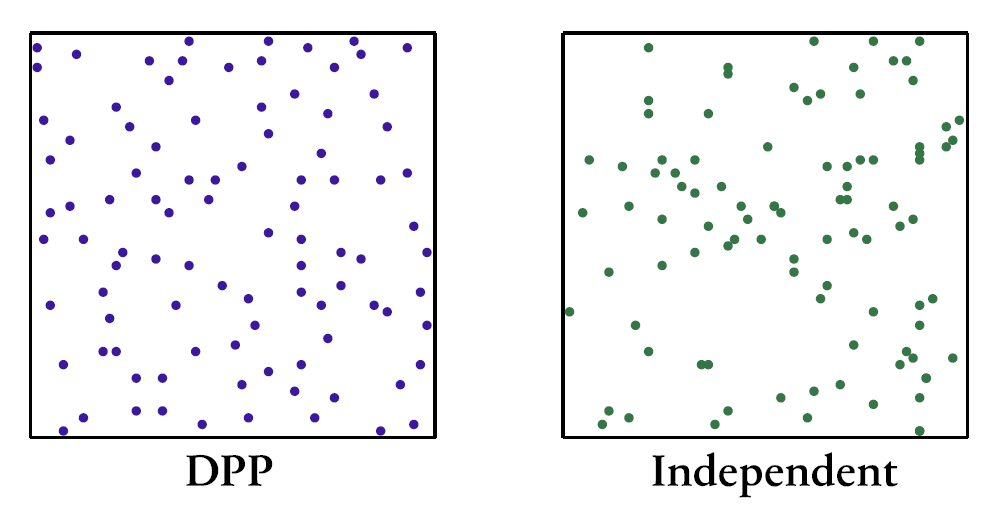
\includegraphics[width=0.6\linewidth]{pics/dpp_vs_iid.png}
    \caption{(left) A set of points in the plane drawn from a DPP, with $K_{i j}$ inversely related to the distance between points $i$ and $j$. (right) The same number of points sampled independently using a Poisson point process , which results in random clumping.}
    \label{fig_dpp_vs_iid}
\end{figure}



\section{Geometric interpretation}
DPP are defined on determinants, that have an intuitive geometric interpretation. Since the DPP kernel $K$ is symmetric, it exists $V \in \RR^{d \times n}$ such that $K= V V\T$. 
Denote the columns of $V$ by $(V_i)$ for $i\in \intint{1}{n}$. Then $\forall A \subseteq \mathcal{X}$

\begin{equation}
    \PP{}{A \subseteq \mathcal{S}} = \operatorname{Vol}^2(V_A)
\end{equation}

The right hand side is the squared $|A|$-dimensional volume of the parallelepiped
spanned by the columns of $V$ corresponding to elements in $A$.

Intuitively, we can think of the columns of $V$ as feature vectors describing the elements
of $\mathcal{X}$. Then the kernel $K$ measures similarity using dot products between feature vectors, and Definition \ref{def_dpp} says that the probability assigned by a DPP to the inclusion of a set $A$ is related to the volume spanned by its associated feature vectors. This is illustrated in Figure \ref{fig_geometric_interpret}.

\begin{figure}[!ht]
    \centering
    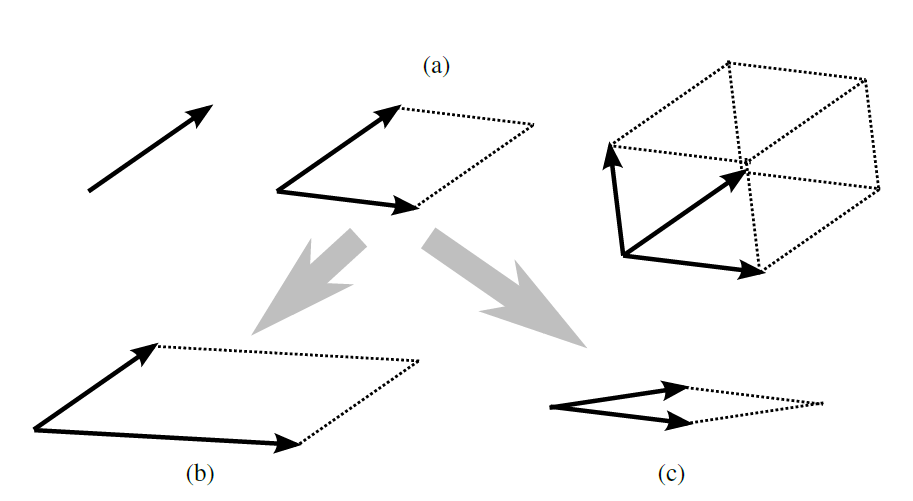
\includegraphics[width=0.8\linewidth]{pics/geometric_interpret.png}
    \caption{A geometric interpretation: each vector corresponds to an element of $\mathcal{X}$. (a) The  probability of inclusion of a subset $A$ is the square of the volume spanned by its associated feature vectors. (b) As the magnitude of an item's feature vector increases, so do the probabilities of sets containing that item. (c) As the similarity between two items increases, the probabilities of sets containing both of them decrease.}
    \label{fig_geometric_interpret}
\end{figure}

This geometric interpretation explain why diverse sets are more probable. It is because their feature vectors are more orthogonal, and hence span larger volumes. Conversely, items with parallel feature vectors are selected together with probability zero, since their feature vectors define a degenerate parallelepiped. Ceteris paribus, items with large magnitude feature vectors are more likely to appear, because the spanned volume for sets containing them evolves linearly with respect to their magnitude, and thus the probability evolves quadratically with respect to it.


\section{Some useful properties}
projection DPP

despite exponential support




\section{Sampling from a DPP}
\subsection{Exact DPP sampling}


Although DPP can be impressively efficient given the exponential number of subsets being sampled from, sampling can be rapidly limited by performance. 
Except for a few specialised kernels like the edges in uniform spanning trees mentioned previously, the default exact sampler is a spectral algorithm due to \cite{hough2006_hkpv}.

It leverages the fact that DPP are mixtures of projection DPP to generate repeated samples given the spectral content of the kernel. This method is commonly called the spectral method since it requires the spectral/eigendecomposition of the positive kernel. 

Formally, if a DPP is defined by a kernel $K$ defined on $n$ data points, one requires the eigendecomposition $K= V V\T$  where $V \in \RR^{d \times n}$. 
This can often be the computational bottleneck since it generally requires $O(n^3)$ time. Note however that for some DPP based on specific kernels like OPE kernels, $K$ is built via this decomposition and thus it is trivially known.

In any cases when multiple samples are required, this eigendecomposition can be reused. Then each sample from the spectral algorithm requires only $O(n k^2)$ time, where $k$ is the number of elements sampled. This means $O(n (\operatorname{Tr} K)^2)$ time on average. If $K$ is a projection kernel, $k = \operatorname{Tr} K = d$ which is a constant than can be small in many practical applications, e.g. in a recommendation context, $k$ would often be less than 10.

Some recent works from \cite{gillenwater2019_treebased_fast_dpp_sampling} improved somewhat this complexity. Based on the still needed eigendecomposition, it implements a binary tree structure storing appropriate summary statistics of the eigenvectors, requiring $O(n d^2)$ to build, but can then generate repeated
samples in $O(\log(n)k^2d^2 + d^3)$ time, hence $O(\log(n)d^4)$ for a projection kernel.

This method becomes a viable alternative to the spectral method when the total
number of items $n$ is large and when the dimensionality $d$ of the
features and the expected sample size $\operatorname{Tr} K$ are small compared to $n$.





\subsection{Approximate DPP sampling}
Several sampling methods have been developed in the case we only need an approximated DPP sampling.

A first class of methods involves a kernel approximation of an given DPP kernel, using random projections such as in \cite{kulesza2012_dpp_for_ml}, or low-rank factorization techniques.

A second class involves Monte Carlo Markov Chain (MCMC). This is often down in an inexact fashion using target distribution close but different from DPP one. Noticeably, \cite{gautier2017_zonotope_for_dpp_sampling} proposed an exact MCMC
sampler for projection DPP.

\vspace{10cm}

\chapter{Correlated importance sampling}
\label{chap_correlated_sampling}



We saw in \cref{chap_DPP} that DPPs is a restriction of correlated sampling that admits useful tractability properties. Moreover, DPPs still maintain expressiveness into the sub-category of negatively correlated sampling, which is the kind of processes we expect to perform better for sample complexity. The intuition is that negatively correlated sampling can eliminate redundancy in sampling sets, an independent sampling can not.

In this chapter, we present current results on coreset sampling with DPPs, and show qualitative results on variance reduction from DPPs. 



\section{A first result with DPPs}


\cite{tremblay2018dppcoreset} first introduce DPPs into the coreset problems, based on the idea of diversity sampling. Their results holds for both DPPs and $m$-DPPs. Since projective DPPs are precisely the intersection of both DPPs and $m$-DPPs, all results apply to them. For the sake of conciseness, we state here their result for $m$-DPPs and we refer to their article for the DPP case.

\begin{tcolorbox}
	\begin{theorem}[From \cite{tremblay2018dppcoreset}]
		Let $(K_m)_{m\in \NN}$ be a sequence of $m$-DPP kernel and let sample $\mathcal{S} \sim \mathcal{DPP}(K_m)$. Assume that the query space $\qset$ is parametrized by some $\theta \in \Theta$, and that all Lipschitz constant with respect to $\theta$ of $\query_\theta \in \qset$ are bounded by some $\lipschitz>0$.\\
		If the minimal sensitivity $\min_{x\in \mathcal{X}}\sigma(x) \geq 1/n$, then for all $\epsilon, \delta \in [0,1]$ 
		\begin{equation*}
            m \geq \frac{32}{\epsilon^{2}}\left(\max_{x\in \mathcal{X}}\frac{m\sigma(x)}{K_m(x,x)}\right)^2 \log \frac{4\eta}{\delta}
			\implies 
			\text{$\mathcal{S}$ is $1-\delta$-surely an $\epsilon$-coreset for $\qset$}
		\end{equation*}
		where $\eta$ is the minimal number of balls of radius $\frac{\epsilon \inf_{f}\loss{f}}{6 n \lipschitz}$ necessary to cover $\Theta$.
	\end{theorem}
\end{tcolorbox}
Note first that the fraction $\frac{m}{K_m(x,x)}$ appearing in the right hand side of the bound is due to the correlated importance sampling framework. This fraction does not appear in the i.i.d. framework because the numerator $m$ cancel with the marginal intensity $mq(x)$. In practice, this fraction can be bounded uniformly on $m$, because $K_m(x,x)$ would typically grow linearly with $m$.

Also note that typically $\log \eta = \OO\left(\pdim \log \frac{n}{\epsilon \inf_{f}\loss{f}}\right)$ with $\pdim = \operatorname{pdim}\qset$, and therefore is dependant on $n$ and $\epsilon$.


Thus, the obtained bound for DPPs does not improve the sample complexity bound for coreset in the i.i.d. framework. The reason is two kind. 

\begin{itemize}
	\item First, the concentration for fixed query is dependant of known concentration results for strongly Rayleigh measures from \cite{pemantle2011rayleighconcentration}, and especially for DPPs. 

	However, one important fact is that it doesn't rely on more advanced concentration for DPPs from \cite{breuer2013nevai} that involves the variance of the estimator. Since recent results from \cite{bardenet2020mcdpp}, it is known DPPs can improve variance rate, and we hope this result to be leveraged into an improved bound on coreset for fixed query.
	\item Second, the generalization to all queries argument that is made introduce a $\log \epsilon^{-1}$ term, and foremost a dependency in $n$, through $\eta$. If not tackled, this could ruin the effort finding improved bound for fixed queries. An improvement way would be to extend classical VC theory arguments in a correlated context.
\end{itemize}


Despite these mitigated results on concentrations, DPPs has already been shown to preform variance reduction, e.g. \cite{bardenet2020mcdpp}.
In the following \cref{sec__variance_arguments}, we present qualitative variance reductions in favour of DPP and $m$-DPP sampling, against Bernoulli process sampling and multinomial sampling.


\section{Variance arguments}
\label{sec__variance_arguments}
We express variance formulas in four sampling cases: multinomial, DPP, Bernoulli process, and $m$-DPP. Then we compare these variances under a domination criteria.
\subsection{Four sampling cases}
\label{subsec__foursampl}
\paragraph{In the multinomial case}, we have $\mathcal S \sim \mathcal M(m, q)$. Then an unbiased estimator of $L$ is
\begin{equation*}
	\estloss{\textrm{iid}}{\query} := \sum_{x\in \mathcal S} \frac{\query(x)}{m q(x)}
\end{equation*}
and its variance is
\begin{equation*}
	\Var{\textrm{iid}}{\query} :=\frac{1}{m} \Var{}{\frac {\query(x)} {q(x)}}
	=\frac{1}{m} \sum_{x \in \mathcal{X}} \frac{\query(x)^{2}}{q(x)} -\frac{1}{m} \loss{\query}^{2} = \boldsymbol\query\T(\frac{Q^{-1}} m - \frac{\moones} m)\boldsymbol\query
\end{equation*}
where $\boldsymbol\query := (f(x))_{x\in \mathcal{X}}$, $Q := \operatorname{diag}(q)$ and $\moones := \voones \voones \T$ the matrix full of ones. 


\paragraph{In the DPP case}, we have $ \mathcal S \sim \mathcal{DPP}(K)$, and for all $x \in \mathcal{X}$, we denote its marginals $\pi_x := K_{xx}$. Then an unbiased estimator of $L$ is
\begin{equation*}
	\estloss{\textrm{DPP}}{\query} := \sum_{x\in \mathcal S} \frac{\query(x)}{\pi_x}
\end{equation*}
Its variance can be computed using $\epsilon_x$ as the counting variable for $x$
\begin{align*}
	\Var{\textrm{DPP}}{\query}
:=\sum_{x,y \in \mathcal{X}}\EE{}{\epsilon_{x} \epsilon_{y}} \frac{\query(x) \query(y)} {\pi_{x} \pi_{y}}  - \loss{\query}^{2}\\
\quad \text{with} \quad
\EE{}{\epsilon_{x} \epsilon_{y}}=
\begin{cases}
	\det K_{\{x, y\}}=\pi_{x} \pi_{y}-K_{xy}^{2}, & \text{if } x \neq y \\
	\EE{}{\epsilon_{x}}=\pi_{x},&\text{if } x = y
\end{cases}
\end{align*}



Introducing $\Pi := \operatorname{diag}(\pi)$ and $\tilde K := \Pi^{-1}K^{\odot 2} \Pi^{-1}$, we can rewrite  

\begin{equation}
	\Var{\textrm{DPP}}{\query}=\sum_{x \in \mathcal{X}}\left(\frac{1}{\pi_{x}}-1\right) \query(x)^{2}-\sum_{x \neq y} \frac{K_{xy}^{2}}{\pi_{x} \pi_{y}} \query(x) \query(y) =  \boldsymbol\query\T (\Pi^{-1}  - \tilde{K}) \boldsymbol\query 
\end{equation}

\paragraph{In the Bernoulli process case}, where for all $x \in \mathcal{X}$, $\PP{}{x \in \mathcal S} = \pi_x$ independently, we have a special case of DPP, where the kernel reduces to its diagonal, i.e. $K = \Pi$ and then $\tilde K = I$. We denote its variance $\Var{\textrm{diag}}{f} := \boldsymbol\query\T (\Pi^{-1}  - I) \boldsymbol\query $.


\paragraph{In the m-DPP case}, we have $\mathcal S \sim \mathcal{DPP}(K) \mid |S|=m$, and we denote its marginals $b_{x} := \mathbb{E}\left[\epsilon_{i}\right]$, that admit an analytic form one can find in \cite{kulesza2012_dpp_for_ml}. Then an unbiased estimator of $L$ is
\begin{equation*}
	\estloss{\textrm{mDPP}}{\query} := \sum_{x\in \mathcal S} \frac{\query(x)}{b_x}
\end{equation*}

and its variance is
\begin{equation}
	\Var{\textrm{mDPP}}{\query}:=\sum_{i}\left(\frac{1}{b_x}-1\right) \query(x)^2
	+ \sum_{x \neq y} C_{xy}\query(x) \query(y)
\end{equation}
where $C_{xy}:=\frac{\mathbb{E}\left[\left(\epsilon_{x}-b_{y}\right)\left(\epsilon_{y}-b_{y}\right)\right]}{\mathbb{E}\left[\epsilon_{i}\right] \mathbb{E}\left[\epsilon_{j}\right]}=\frac{\mathbb{E}\left[\epsilon_{x} \epsilon_{y}\right]}{b_{x} b_{y}}-1
$

Observe that if the m-DPP kernel is reduced to its diagonal ($C_{xy} = 0$), we recover $\Var{\textrm{diag}}{}$, the variance of a Bernoulli process with same marginals ($\pi_x = b_x$), though the former has fixed sample size $m$, and the latter not.

In order to benefit from some variance reduction, one should find a $m$-DPP where $\forall x\neq y \,,\, C_{xy}\query(x) \query(y) <0$.

\cite{zhang2017dppminibatch} discuss that intuitively, if the $m$-DPP kernel rely on some similarity measure and that $f$ is smooth for it, then 2 similar points should have both negative correlation ($C_{xy}<0$) and their value have positive scalar product ($\query(x) \query(y) > 0$). This provides variance reduction.

Reversely, they argued that 2 dissimilar points should have positive correlation, and their value show ``no tendency to align'' hinting $\query(x) \query(y) < 0$, and again providing variance reduction. However, properties of strong Rayleigh measures implies always $C_{xy}\leq0$ (see \cite{pemantle2011rayleighconcentration}). But we could more conservatively consider that, whether DPP or $m$-DPP, two dissimilar points tend toward independence. Thus the induced variance change, whether positive or negative depending on the sign of $\query(x) \query(y)$, would in either case be small. 



\subsection{Variance comparison}
In the following, we compare processes with same marginals, and therefore set $\Pi = mQ$. Also, 
since $m$-DPP marginals admits analytic but complicated form, we drop the $m$-DPP case comparison. We show in \cref{subsec__foursampl} that $\Var{\textrm{iid}}{}$, $\Var{\textrm{diag}}{}$ and $\Var{\textrm{DPP}}{}$ are quadratic forms of $\boldsymbol\query$ associated with respective matrices
$$\begin{cases}
	\Var{\textrm{iid}}{} \equiv \Pi^{-1} - \frac{\moones}{m} \\
	\Var{\textrm{diag}}{} \equiv \Pi^{-1} - I \\
	\Var{\textrm{DPP}}{} \equiv \Pi^{-1} - \tilde K
\end{cases}$$

This allows to compare samplings through the Loewner ordering ($\preceq$) of the variance associated matrices. For instance, we say DPP variance strictly dominates Bernoulli process variance if it uniformly yields lower variance, which is equivalent to $\tilde K$ being strictly greater than identity. Formally 
\begin{equation*}
	\forall \query \in \RR^{\mathcal{X}}, \, \Var{\textrm{DPP}}{f} < \Var{\textrm{diag}}{f} \iff \tilde K \succ I.
\end{equation*}
Massaging some linear algebra thus gives

\begin{tcolorbox}
	\begin{proposition}[Variance comparison]\ \\
		\label{prop__var_comp}
		DPP variance dominates Bernoulli process variance on positive-valued functions
		\begin{align}
			\label{eqn__posvar}
			\forall \query \in \RR_+^{\mathcal{X}},\ \Var{\textrm{DPP}}{f} \leq \Var{\textrm{diag}}{f}.
		\end{align}
		In the general case of real-valued functions, DPP variance does not dominate Bernoulli process variance but does up to a factor three
		\begin{align}
			\label{eqn__nodom}
			&\exists \query \in \RR^{\mathcal{X}},\ \Var{\textrm{DPP}}{f} \geq \Var{\textrm{diag}}{f}\\
			\label{eqn__domtwo}
			&\forall \query \in \RR^{\mathcal{X}},\ \Var{\textrm{DPP}}{f} \leq 3\Var{\textrm{diag}}{f}.
		\end{align}
		Moreover, if the DPP is projective, then
		\begin{align}
			\label{eqn__projiid}
			\forall \query \in \RR^{\mathcal{X}},\ \Var{\textrm{DPP}}{f} \leq \Var{\textrm{i.i.d.}}{f}.
		\end{align}
	\end{proposition}
\end{tcolorbox}



\begin{proof}[Proof of:]\
	\begin{enumerate}
		\item[\cref{eqn__posvar}] Assume $\query \in \RR_+^{\mathcal{X}}$. Then $\boldsymbol\query\T (\tilde K - I)\boldsymbol\query = \sum_{x \neq y} \frac{K_{xy}^{2}}{\pi_{x} \pi_{y}} \query(x) \query(y) \geq 0$ and therefore $\Var{\textrm{DPP}}{f} \leq \Var{\textrm{diag}}{f}$.
		\item[\cref{eqn__nodom}] $\tilde K = \Pi^{-1}K^{\odot 2} \Pi^{-1}$ is a symmetric positive matrix and by Hadamard inequality $\det( \tilde K) \leq \prod_{x\in \mathcal{X}} \tilde K_{xx}= 1$. Therefore at least one of its eigenvalue is lower than 1, hence $\tilde K \nsucc I \iff \exists \query \in \RR^{\mathcal{X}},\ \Var{\textrm{DPP}}{f} \geq \Var{\textrm{diag}}{f}$.
		\item[\cref{eqn__domtwo}]
			For all $f\in \RR^{\mathcal{X}}$, let denote by $f = f_+ - f_-$ its decomposition into its positive and negative part, which both belong in $\RR_+^{\mathcal{X}}$. Then we have

		\begin{align*}
			\hspace{-1cm}\Var{\textrm{DPP}}{f} &= \Var{\textrm{DPP}}{f_+} + \Var{\textrm{DPP}}{f_-} - 2\Cov{\textrm{DPP}}{f_+,f_-} \ &\text{\footnotesize Al-Kashi}\\
			&\leq \Var{\textrm{DPP}}{f_+} + \Var{\textrm{DPP}}{f_-} + 2\sqrt[]{\Var{\textrm{DPP}}{f_+}\Var{\textrm{DPP}}{f_-}} \ &\text{\footnotesize Cauchy-Schwartz}\\
			&\leq \Var{\textrm{diag}}{f_+} + \Var{\textrm{diag}}{f_-} + 2\sqrt[]{\Var{\textrm{diag}}{f_+}\Var{\textrm{diag}}{f_-}} \ &\text{\footnotesize \cref{eqn__posvar}}\\
			&\leq 3\Var{\textrm{diag}}{f}
		\end{align*}

		where we lastly use that $\Var{\textrm{diag}}{f} = \Var{\textrm{diag}}{f_+} + \Var{\textrm{diag}}{f_-}$ since its associated matrix is diagonal.
		\item[\cref{eqn__projiid}]
		$K$ being symmetric positive of rank $r \in \intint{0}{n}$, it exists $V \in \RR^{r \times n}$ such that $K = V\T V$, and we denote by $V_i$ its colons, for $i \in \intint{1}{n}$.
	
		For any vector $v \in \RR^{r}$, \cite{copenhaver2013diagramvectors} define its diagram vector 
		$$\tilde v :=
			\frac{1}{\sqrt{r-1}} (v_k^{2}-v_l^{2} , \sqrt{2 r} v_k v_l )_{k<l}\T \in \RR^{r(r-1)}$$
		concatenating all the $\frac{r(r-1)}{2}$ differences of squares and $\frac{r(r-1)}{2}$ products.
		
		Then introduce $\tilde V = (\tilde V_i )_{i\in\intint{1}{n}}$, the matrix whose columns are diagram vectors of matrix $V$ columns. It allows us to rewrite $\tilde K = \frac{\moones}{r} + \frac{r-1}{r} \tilde V\T \tilde V$ thus $\tilde K - \frac{\moones}{m} = (\frac{1}{r}-\frac{1}{m})\moones + \frac{m-1}{m} \tilde V\T \tilde V$. Then in order to have 
		\begin{equation*}
			\tilde K - \frac{\moones}{m}\succeq 0 \iff \forall \query \in \RR^{\mathcal{X}},\ \Var{\textrm{DPP}}{f} \leq \Var{\textrm{i.i.d.}}{f}
		\end{equation*}
		it is sufficient to have DPP kernel $K$ such that $r \leq m$. On the other hand, we know its average number of samples is $\operatorname{Tr}K = \operatorname{Tr}\Pi^{-1} = m$, because we fixed its marginals. Moreover $\operatorname{Tr}K \leq r$ holds for every DPP, this implies $\operatorname{Tr}K=r$, and therefore it is a projective DPP. Put differently, for any multinomial sampling, we have a projective DPP that beats it uniformly.
	\end{enumerate}
	
\end{proof}

Note that \cref{eqn__domtwo} use the general inequality
\begin{equation*}
	\Var{}{f} \leq \Var{}{f_+} + \Var{}{f_-} + 2\sqrt[]{\Var{}{f_+}\Var{}{f_-}}
\end{equation*}
which justifies that in many cases, we can restrict ourselves to controlling variances of positive-valued functions without loss of generality.

In the case of positive valued functions, \cref{prop__var_comp} shows that for any Bernoulli process or multinomial sampling, taking any projective DPP sampling with same marginals would yield lower variance. This is a strong qualitative argument for the use of projective DPPs for the coreset problem, that we will now try to quantify.



\printbibliography
%	 \bibliographystyle{chicago}
%	 \bibliography{biblio.bib}
\end{document}